%% TIKZ DRAWING OF CALIFES ELEMENTS
%% TO BE INCLUDED INTO A LATEX DOCUMENT
%% K. Sjobak, 2018

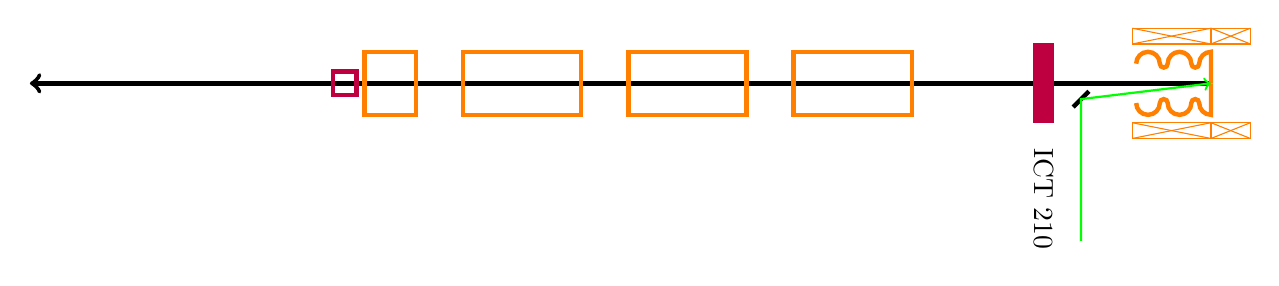
\begin{tikzpicture}
    \draw[<-,ultra thick] (0,0)--(15,0);
    
    %% GUN
    
    % Gun solenoids
    \draw[orange] (15,0.5) rectangle (14,0.7);
    \draw[orange] (15,0.5) -- (14,0.7);
    \draw[orange] (15,0.7) -- (14,0.5);
    \draw[orange] (15,-0.5) rectangle (14,-0.7);
    \draw[orange] (15,-0.5) -- (14,-0.7);
    \draw[orange] (15,-0.7) -- (14,-0.5);
    
    \draw[orange] (15.5,0.5) rectangle (15,0.7);
    \draw[orange] (15.5,0.5) -- (15,0.7);
    \draw[orange] (15.5,0.7) -- (15,0.5);
    \draw[orange] (15.5,-0.5) rectangle (15,-0.7);
    \draw[orange] (15.5,-0.5) -- (15,-0.7);
    \draw[orange] (15.5,-0.7) -- (15,-0.5);
    
    % Gun cavity
    \draw[orange, ultra thick] (15,0.0) to (15,0.4)
        arc(90:180:0.15)
        arc(360:180:0.05) arc(0:180:0.15)
        arc(360:180:0.05) arc(0:180:0.15);
    \draw[orange, ultra thick] (15,0.0) to (15,-0.4)
        arc(-90:-180:0.15)
        arc(0:180:0.05) arc(0:-180:0.15)
        arc(0:180:0.05) arc(0:-180:0.15);
    
    \correctorMagnet{13.7}{DG 130};
    
    %Laser mirror    
    \draw[ultra thick]  ({(13.7-13)/2+13 + 0.1}, -0.1) --
                        ({(13.7-13)/2+13 - 0.1}, -0.3);
%    \draw[thick,->,green] ({(13.7-13)/2+13-0.2},{-(15-((13.7-13)/2+13))}) --
%                          ({(13.7-13)/2+13},-0.2) -- 
%                          (15,0);
    \draw[thick,->,green] ({(13.7-13)/2+13},-2) --
                          ({(13.7-13)/2+13},-0.2) -- 
                          (15,0);
    
    
    \filldraw[purple] (13.,-0.5) rectangle (12.75,0.5);
    \node[rotate=-90,anchor=west] at (12.75+0.25/2,-0.7) {ICT 210};

    \BTV{12.25}{MTV 215}
    
    \cBPM{11.6}{BPM 220}
    \correctorMagnet{11.35}{DG 225};
    
    \draw[ultra thick, orange] (11.2,-0.4) rectangle (9.7,0.4);
    \cBPM{9.5}{BPM 240}
    \correctorMagnet{9.25}{DG 245};
    
    \draw[ultra thick, orange] (9.1,-0.4) rectangle (7.6,0.4);
    \cBPM{7.4}{BPM 260}
    \correctorMagnet{7.15}{DG 265};
    
    \draw[ultra thick, orange] (7.0,-0.4) rectangle (5.5,0.4);
    \cBPM{5.3}{BPM 310}
    \correctorMagnet{5.05}{DG 320};
    
    \draw[ultra thick, orange] (4.9,-0.4) rectangle (4.25,0.4);
    
    \draw[ultra thick, purple] (4.15,-0.15) rectangle (3.85,0.15);
    
    \lensF{3.5}{QFD 350};
    \lensD{3.0}{QDD 355};
\end{tikzpicture}